\documentclass[11pt,letterpaper,twoside]{book}

% ==========================================
% SIRCUS System Manual
% How the SIRCUS console is put together: clocks, bus, interrupts, reset, connections and timing
% ==========================================

% Manual-specific strings used by the shared preamble (footer, PDF metadata).
\newcommand{\sircManualFooter}{SIRCUS SYSTEM MANUAL}
\newcommand{\sircManualTitle}{SIRCUS System Manual}
\newcommand{\sircManualSubject}{SIRCUS, the SIRC User System: clocks, bus, interrupts, reset, connections and timing}

% Names of this manual and its siblings, for references within the set.
\newcommand{\sysmanual}{\textit{SIRCUS System Manual}}
\newcommand{\audiomanual}{\textit{SIRCAS Reference Manual}}
\newcommand{\videomanual}{\textit{SIRCADA Reference Manual}}

% ==========================================
% Shared preamble for the SIRC-1 manuals (docs/reference and docs/hardware)
% ==========================================

% ------------------------------------------------------------
% Encoding and typography
% ------------------------------------------------------------

\usepackage[utf8]{inputenc}
\usepackage[T1]{fontenc}

% Helvetica-compatible sans serif.
% TeX Gyre Heros is a high-quality Helvetica replacement.
\usepackage{tgheros}
\renewcommand{\familydefault}{\sfdefault}

% Courier-compatible monospace.
\usepackage{tgcursor}

% Better character spacing / kerning.
\usepackage{microtype}

% ------------------------------------------------------------
% Page layout
% ------------------------------------------------------------

\usepackage{geometry}

\geometry{
	a4paper,
	left=25mm,
	right=20mm,
	top=22mm,
	bottom=25mm,
	headheight=14pt
}

% The book class flushes page bottoms in two-sided mode. With many [H] tables
% that cuts pages short, so the leftover space gets spread through lists and
% paragraphs instead. Let short pages stay short.
\raggedbottom

% ------------------------------------------------------------
% General packages
% ------------------------------------------------------------

\usepackage{graphicx}
\usepackage{eso-pic}
\usepackage{xcolor}
\usepackage{fancyhdr}
\usepackage{titlesec}
\usepackage{enumitem}
\usepackage{float}

% A captioned, non-floating environment for worked assembly examples, so
% they get a real "List of Examples" (like the existing List of
% Figures/Tables) instead of a hand-maintained one. Numbered N-M (chapter
% number, then sequential within that chapter/appendix) to match the
% manual's existing "Example 13-1" convention; [H] means it never actually
% floats away from where the author placed it.
\newfloat{example}{H}{loe}[chapter]
\floatname{example}{Example}
\renewcommand{\theexample}{\thechapter-\arabic{example}}

\usepackage{tabularx}
\usepackage{booktabs}
\usepackage{multirow}
\usepackage{longtable}
\usepackage{xltabular}

\usepackage{amsmath}
\usepackage{amssymb}

\usepackage{listings}
\usepackage{bytefield}
\bytefieldsetup{endianness=big}

\usepackage{tikz}
\usepackage{tikz-timing}
\usetikzlibrary{
	shapes.geometric,
	arrows.meta,
	positioning,
	fit,
	calc
}

\usepackage{tcolorbox}
\tcbuselibrary{breakable, skins}

% Load hyperref relatively late.
\usepackage{hyperref}

% ------------------------------------------------------------
% Timing diagrams
% ------------------------------------------------------------

\tikzset{
	sirc timing diagram/.style={
			timing/slope=0,
			timing/dslope=0.15,
			timing/xunit=3.4em,
			timing/rowdist=2.2,
			timing/coldist=2.2,
		},
}

% ------------------------------------------------------------
% Colours
% ------------------------------------------------------------

\definecolor{sircred}{RGB}{255,0,0}
\definecolor{sircgray}{RGB}{110,110,110}
\definecolor{sirclightgray}{RGB}{232,232,232}
\definecolor{codebg}{RGB}{245,245,245}
\definecolor{opcodecolor}{RGB}{153,0,0}

% ------------------------------------------------------------
% Manual-specific strings
% ------------------------------------------------------------
% A manual's main.tex defines these (with \newcommand) before it inputs this
% preamble. The defaults are for the Architecture Reference Manual.

\providecommand{\sircManualFooter}{SIRC-1 ARCHITECTURE REFERENCE MANUAL}
\providecommand{\sircManualTitle}{SIRC-1 Architecture Reference Manual}
\providecommand{\sircManualSubject}{SIRCIS Instruction Set Architecture}

% Names of the manuals in the set, for references between them
\providecommand{\archmanual}{\textit{SIRC-1 Architecture Reference Manual}}
\providecommand{\hwmanual}{\textit{SIRC-1 Hardware Reference Manual}}
\providecommand{\asmmanual}{\textit{SIRC-1 Assembly Programmer's Manual}}

% ------------------------------------------------------------
% Header / footer
% ------------------------------------------------------------

\pagestyle{fancy}
\fancyhf{}

\fancyhead[LE]{\small\nouppercase{\leftmark}}
\fancyhead[RO]{\small\nouppercase{\rightmark}}
\fancyhead[RE,LO]{\small\textcolor{sircred}{DRAFT --- Not for Distribution}}

\fancyfoot[LE,RO]{\thepage}
\fancyfoot[C]{\small\textcolor{sircgray}{\sircManualFooter}}

\renewcommand{\headrulewidth}{0.8pt}
\renewcommand{\footrulewidth}{0.4pt}

% ------------------------------------------------------------
% PDF / hyperlink setup
% ------------------------------------------------------------

\hypersetup{
	colorlinks=true,
	linkcolor=sircred,
	filecolor=sircred,
	urlcolor=sircred,
	citecolor=sircred,
	bookmarksnumbered=true,
	pdfauthor={SIRC Development Team},
	pdftitle={\sircManualTitle},
	pdfsubject={\sircManualSubject},
}

% ------------------------------------------------------------
% Assembly code listings
% ------------------------------------------------------------

\lstdefinelanguage{SIRC}{
	morekeywords={
			ADDI,ADDR,ADCI,ADCR,SUBI,SUBR,SBCI,SBCR,
			ANDI,ANDR,ORRI,ORRR,XORI,XORR,
			LOAD,MOVI,MOVR,STOR,CMNI,CMNR,CNCI,CNCR,CMPI,CMPR,CPCI,CPCR,TSAI,TSAR,TSOI,TSOR,TSXI,TSXR,
			LDEA,LDEL,BRAN,LJMP,LJSR,BRSR,RETS,NOOP,
			WAIT,RETE,COPI,COPR,SHFT,EXCP,RSET,
			ETFR,ETTR,DMAR,DMAW,DMAT,MULU,MULS,DIVU,DIVS
		},
	keywordstyle=\color{sircred}\bfseries,
	sensitive=false,
	morecomment=[l]{;},
	commentstyle=\itshape\color{sircgray},
	morestring=[b]",
	stringstyle=\color{opcodecolor},
	basicstyle=\ttfamily\small,
	breaklines=true,
	showstringspaces=false
}

\lstset{
	language=SIRC,
	backgroundcolor=\color{codebg},
	frame=single,
	rulecolor=\color{sircgray},
	framesep=5pt,
	numbers=left,
	numberstyle=\tiny\color{sircgray},
	numbersep=7pt,
	xleftmargin=15pt,
	framexleftmargin=15pt,
	columns=fullflexible
}

% ------------------------------------------------------------
% Instruction reference pages
% ------------------------------------------------------------

% Modelled on the instruction-description pages of period CPU manuals (e.g.
% the M68000 Family Programmer's Reference Manual): each instruction gets a
% dedicated page (or run of pages) with the mnemonic set prominently at the
% top for flip-through lookup, rather than a boxed callout sitting in the
% middle of running text. \clearpage at the start of every entry guarantees
% two entries never share a page -- if one entry runs long, the next simply
% starts on the page after it ends. The chapter running header (already set
% by fancyhdr) carries the instruction category, matching how the M68000
% manual shows its category ("Integer Instructions", etc.) in the header of
% every instruction page.
%
% Every entry also gets its own table-of-contents/PDF-bookmark line, keyed
% off its own mnemonic and name, regardless of whether it sits directly
% under a \section of its own or is one of several instructions grouped
% under a shared \section (e.g. the Exception Unit meta-instructions in
% Chapter 16) -- so every instruction is individually findable via the ToC
% or bookmarks either way, matching the "flip through to find it" goal.
\newenvironment{instructionbox}[2]{%
	\clearpage
	\phantomsection
	\addcontentsline{toc}{section}{#1 -- #2}
	\noindent{\Huge\bfseries\color{sircred}#1}\par
	\vspace{3pt}
	\noindent{\Large\bfseries #2}\par
	\vspace{6pt}
	\titlerule
	\vspace{10pt}
}{%
}

% A compact boxed reference for one addressing mode: GENERATION, ASSEMBLER
% SYNTAX, FIELD ENCODING, and INSTRUCTION WORD COUNT, matching the M68000
% PRM's per-mode encoding box. Unlike instructionbox, this does not force a
% page break -- there are only seven addressing modes and each is short
% enough that several fit per page.
\newtcolorbox{addrmodebox}[1]{
	colback=sirclightgray,
	colframe=sircred,
	coltitle=black,
	fonttitle=\bfseries\large,
	title=#1,
	arc=0mm,
	boxrule=0.8pt,
	breakable,
	enhanced jigsaw,
}

% ------------------------------------------------------------
% Architectural notation
% ------------------------------------------------------------

\newcommand{\reg}[1]{\texttt{#1}}
\newcommand{\opcode}[1]{\textcolor{opcodecolor}{\texttt{0x#1}}}
\newcommand{\statusbit}[1]{\texttt{#1}}
\newcommand{\mnemonic}[1]{\textbf{\texttt{#1}}}
\newcommand{\addr}[1]{\texttt{#1}}
\newcommand{\imm}[1]{\texttt{\##1}}

\newcommand{\indirectimm}[2]{\texttt{(\##1, #2)}}
\newcommand{\indirectreg}[2]{\texttt{(#1, #2)}}
\newcommand{\postinc}[2]{\texttt{(#1, #2)+}}
\newcommand{\predec}[2]{\texttt{-(#1, #2)}}

\newcommand{\shift}[2]{\texttt{#1 \##2}}

% Active-low signal name with a period overbar, e.g. \activelow{BERR}
\newcommand{\activelow}[1]{\ensuremath{\overline{\mbox{#1}}}}

% ------------------------------------------------------------
% Chapter / section styling
% ------------------------------------------------------------

% Deliberately simple, mechanical headings rather than modern
% display typography.

\titleformat{\chapter}[display]
{\normalfont\bfseries\color{sircred}}
{\Large CHAPTER \thechapter}
{8pt}
{\Huge}
[\vspace{4pt}\titlerule]

\titlespacing*{\chapter}
{0pt}
{-10pt}
{28pt}

\titleformat{\section}
{\normalfont\Large\bfseries\color{sircred}}
{\thesection}
{1em}
{}

\titleformat{\subsection}
{\normalfont\large\bfseries\color{sircred}}
{\thesubsection}
{1em}
{}

\titleformat{\subsubsection}
{\normalfont\normalsize\bfseries}
{\thesubsubsection}
{1em}
{}

\titlespacing*{\section}
{0pt}
{2.5ex plus 0.5ex minus 0.2ex}
{1ex}

\titlespacing*{\subsection}
{0pt}
{2ex plus 0.5ex minus 0.2ex}
{0.8ex}

% ------------------------------------------------------------
% Tables
% ------------------------------------------------------------

\renewcommand{\arraystretch}{1.2}


\begin{document}

% Front Matter
\frontmatter
\AddToShipoutPictureBG*{%
	\put(0,0){
\includegraphics[width=\paperwidth,height=\paperheight]{../logos/cover-simple.jpg}}%
}

\begin{titlepage}
	\thispagestyle{empty}
	\centering

	\vspace*{2.5cm}

	
\includegraphics[width=0.45\textwidth]{../reference/sirc-logo.png}

	\vspace{0.8cm}

	{\Huge\bfseries\color{black} SIRCUS}

	\vspace{0.3cm}

	{\LARGE\bfseries\color{black} System Manual}

	\vspace{0.4cm}

	{\large\itshape\color{black} SIRC User System: Clocks, Bus, Interrupts, Reset, Connections and Timing}

	\vfill

	{\small\color{black} SILICON INTEGRATED RESEARCH CORPORATION}

	\vspace{1cm}

\end{titlepage}

\chapter*{Preface}
\addcontentsline{toc}{chapter}{Preface}
\label{ch:preface}

\section*{About This Manual}

This manual documents SIRCUS, the SIRC User System: the console built from the SIRC-1 CPU, the SIRCADA display adapter
and the SIRCAS sound processor. The three chips each have a manual of their own, which describes what the chip does and
how it behaves at its pins. This manual describes what the chips do not describe for themselves: how they are
connected, which clock each one runs from, how they share one bus and a small set of interrupt lines, how they are
reset, and how the timing of each one relates to the others.

It is a companion to the \archmanual{}, which defines the CPU's instructions and exceptions, to the \hwmanual{}, which
defines the CPU package and bus, to the \asmmanual{}, which defines the language used to program the system, to the
\videomanual{} and to the \audiomanual{}.

It is written for:

\begin{itemize}
	\item Engineers building the console, who need to know what every pin connects to and how fast
	\item Programmers who need the timing relationships between the picture, the sound and the CPU
	\item Authors of tools and emulators, who must reproduce those relationships
\end{itemize}

\section*{Assumed Knowledge}

This manual assumes the reader has the manual of each chip to hand. It repeats a fact from them only where the fact is
needed to understand the connection, and it names the chapter that holds the full account instead of reproducing it.

\section*{Revision Status}

This is a draft of the \sysmanual{}, not for distribution. Anything not yet decided in the manual is marked ``not yet
specified''; the manual does not invent values for it.

\tableofcontents
\listoftables
\listoffigures

% Main Content
\mainmatter
\chapter{Introduction}
\label{ch:introduction}

\section{Purpose and Scope}

The SIRC-1 CPU is sold on its own, so it is documented in three manuals that stand apart from any system built around
it. SIRCADA and SIRCAS are made for the SIRCUS system and each has a manual of its own. This manual completes the set:
it describes the system that the parts are built into. The six manuals have these scopes:

\begin{table}[H]
	\centering
	\begin{tabular}{lp{8.2cm}}
		\toprule
		\textbf{Manual} & \textbf{Scope}                                                                                               \\
		\midrule
		\archmanual{}   & ISA, instruction encodings, canonical assembly notation, exceptions, programmer-visible state                \\
		\asmmanual{}    & Complete assembly syntax, directives, symbols, meta-instructions, and toolchain usage                        \\
		\hwmanual{}     & Pinout, bus interface, timing, electrical characteristics                                                    \\
		\videomanual{}  & The display adapter: package and pinout, memory map, registers, data formats, video modes, timing            \\
		\audiomanual{}  & The sound processor: package and pinout, memory map, registers, data formats, voices, filter, sequencer      \\
		\sysmanual{}    & The console: clocks, bus, address map, interrupts, reset, connections and timing between chips (this manual) \\
		\bottomrule
	\end{tabular}
	\caption{The SIRC-1 and SIRCUS Manual Set}
	\label{tab:manual-set}
\end{table}

Where a chip's own manual is authoritative for something, this manual says so and names the chapter. Where the
connection of two chips creates a fact that neither manual could state alone, such as the number of audio samples in a
video frame, this manual is authoritative.

\section{The Parts of the System}

SIRCUS has three chips that matter to a program, each on the one 16-bit bus, and the memories and circuits around them.

\begin{table}[H]
	\centering
	\small
	\begin{tabular}{llp{5.2cm}}
		\toprule
		\textbf{Part}     & \textbf{Package}            & \textbf{Function}                                                                               \\
		\midrule
		SIRC-1 CPU        & 64-pin DIP                  & Runs the program; the only master of the bus                                                    \\
		SIRCADA           & 52-pin PLCC                 & Display adapter: tiles, sprites and the video signal; holds its own video memory                \\
		SIRCAS            & Not yet specified           & Sound processor: six voices, filter and sequencers; has its own audio memory                    \\
		Audio memory      & Not yet specified           & Static memory of 32,768 words, used by SIRCAS alone                                             \\
		Converter         & TDA1541A, 28-pin DIP        & Philips dual 16-bit converter: turns SIRCAS's serial output into two analogue currents          \\
		Output amplifiers & Not yet specified           & Turn the converter's currents into voltages (a reference circuit uses two NE5534 or equivalent) \\
		Working memory    & Not yet specified           & 128 KB (65,536 words) of RAM for the program's data and stack                                   \\
		System ROM        & Not yet specified           & Holds the start-up code and the driver routines that programs call                              \\
		Cartridge         & Connector not yet specified & Holds a game's program and data in a ROM; its first words are the reset vector                  \\
		Serial I/O        & MC68681 DUART               & Motorola dual serial port: links two consoles, a modem or a debugger                            \\
		Select logic      & 74LS138, 16-pin DIP         & Decodes A23 to A21 into a chip select for each device; a latch holds the boot overlay           \\
		Clock circuit     & Not yet specified           & Makes the master clock and divides it by two to make \texttt{CLKI}                              \\
		\bottomrule
	\end{tabular}
	\caption{The Parts of SIRCUS}
	\label{tab:parts}
\end{table}

The video memory is inside SIRCADA, and the CPU reaches it through the device's own segment (\videomanual{}, memory map
chapter). The audio memory is outside SIRCAS, but it is not on the CPU's bus: the CPU reaches it only through a window
of SIRCAS's segment, and SIRCAS makes every access to it itself (\audiomanual{}, memory map chapter). The CPU's bus
therefore carries traffic for only six things: the working memory, the system ROM, the cartridge, SIRCADA, SIRCAS and
the serial device.

\section{Block Diagram}

Figure~\ref{fig:block-diagram} shows the connections. One clock rail feeds all three chips, one bus joins them, and
each of the other two chips has outputs that the CPU never sees directly: the picture, and the sound.

\begin{figure}[H]
	\centering
	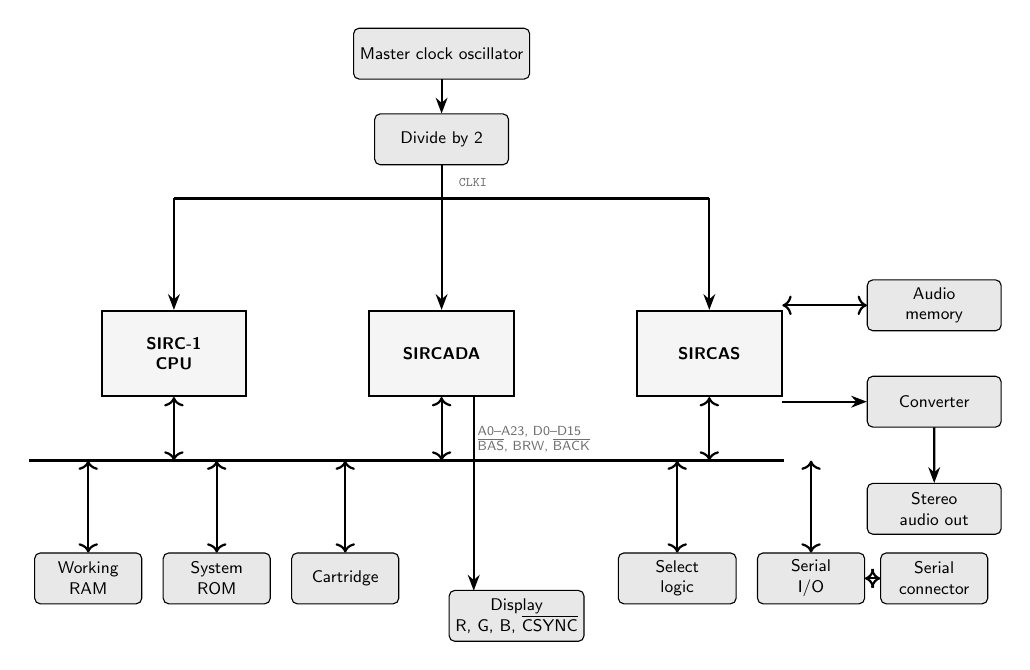
\begin{tikzpicture}[
			scale=0.68, transform shape,
			chip/.style={draw, thick, fill=gray!8, align=center, font=\bfseries\small, minimum width=2.7cm, minimum height=1.6cm},
			box/.style={draw, rounded corners=2pt, fill=sirclightgray, align=center, font=\small, minimum width=2.5cm, minimum height=0.95cm},
			flow/.style={-{Stealth[length=2mm]}, thick},
			rail/.style={very thick},
			note/.style={font=\scriptsize, text=sircgray, align=center}
		]
		% Clock
		\node[box] (osc) at (0,5.6) {Master clock oscillator};
		\node[box] (div) at (0,4.0) {Divide by 2};
		\draw[flow] (osc) -- (div);
		\draw[rail] (-5,2.9) -- (5,2.9);
		\draw[thick] (div.south) -- (0,2.9);
		\node[note, anchor=south west] at (0.2,3.0) {\texttt{CLKI}};
		% Chips
		\node[chip] (cpu) at (-5,0) {SIRC-1\\CPU};
		\node[chip] (ppu) at (0,0) {SIRCADA};
		\node[chip] (snd) at (5,0) {SIRCAS};
		\foreach \c in {cpu,ppu,snd} { \draw[flow] (\c |- 0,2.9) -- (\c.north); }
		% Bus
		\draw[rail] (-7.7,-2.0) -- (6.4,-2.0);
		\foreach \c in {cpu,ppu,snd} { \draw[thick, <->] (\c.south) -- (\c |- 0,-2.0); }
		\node[note, anchor=south west, align=left] at (0.55,-1.97) {A0--A23, D0--D15\\\activelow{BAS}, BRW, \activelow{BACK}};
		% Below the bus
		\node[box, minimum width=2.0cm] (ram) at (-6.6,-4.2) {Working\\RAM};
		\node[box, minimum width=2.0cm] (rom) at (-4.2,-4.2) {System\\ROM};
		\node[box, minimum width=2.0cm] (cart) at (-1.8,-4.2) {Cartridge};
		\node[box, minimum width=2.2cm] (sel) at (4.4,-4.2) {Select\\logic};
		\node[box, minimum width=2.0cm] (ser) at (6.9,-4.2) {Serial\\I/O};
		\node[box, minimum width=2.0cm] (sconn) at (9.2,-4.2) {Serial\\connector};
		\draw[thick, <->] (ser.north) -- (ser |- 0,-2.0);
		\draw[flow, <->] (ser) -- (sconn);
		\foreach \c in {ram,rom,cart,sel} { \draw[thick, <->] (\c.north) -- (\c |- 0,-2.0); }
		% Outputs
		\node[box] (disp) at (1.4,-4.9) {Display\\R, G, B, \activelow{CSYNC}};
		\draw[flow] (0.6,-0.8) -- (0.6,-4.43);
		% Audio side
		\node[box] (amem) at (9.2,0.9) {Audio\\memory};
		\node[box] (dac) at (9.2,-0.9) {Converter};
		\draw[thick, <->] (snd.east |- amem) -- (amem.west);
		\draw[flow] (snd.east |- dac) -- (dac.west);
		\node[box] (out) at (9.2,-2.9) {Stereo\\audio out};
		\draw[flow] (dac) -- (out);
	\end{tikzpicture}
	\caption{SIRCUS Block Diagram}
	\label{fig:block-diagram}
\end{figure}

The interrupt and reset connections are not drawn; Chapter~\ref{ch:interrupts} gives them, and
Chapter~\ref{ch:connections} lists every connection of every chip.

\section{Conventions}

\begin{itemize}
	\item \textbf{Addresses} are word addresses of 24 bits, as in the \hwmanual{}. A segment is 65,536 words, and the
	      eight high address bits select it.
	\item \textbf{Active-low signals} carry a bar over the name and are asserted when low.
	\item \textbf{Clock cycles} are cycles of \texttt{CLKI}, the clock every chip takes, unless a figure says otherwise.
	      The master clock is twice as fast.
	\item \textbf{Both regions.} Figures are given for an NTSC console and a PAL console. A figure without a region
	      holds for both.
	\item \textbf{Not yet specified.} A value that the design has not fixed is marked ``not yet specified''. It is not
	      undefined, and no value is implied.
\end{itemize}

\chapter{Clocks}
\label{ch:clocks}

SIRCUS has one oscillator. Every other rate in the system is that oscillator divided down, so every timing in the
console is a whole number of cycles of it, and the three chips stay in step without any of them watching another.

\section{The Master Clock}
\label{sec:master-clock}

The master clock is the system oscillator. Its frequency depends on the region, because the video signal that SIRCADA
makes must match the colour subcarrier of the television standard:

\begin{table}[H]
	\centering
	\begin{tabular}{lll}
		\toprule
		\textbf{Region} & \textbf{Master clock} & \textbf{Derivation}                 \\
		\midrule
		NTSC            & 21,477,272 Hz         & The NTSC colour subcarrier times 6  \\
		PAL             & 21,281,370 Hz         & The PAL colour subcarrier times 4.8 \\
		\bottomrule
	\end{tabular}
	\caption{The Master Clock}
	\label{tab:master-clock}
\end{table}

The oscillator itself, its tolerance and its drive circuit are not yet specified.

\section{The Clock Rail}
\label{sec:clock-rail}

The system divides the master clock by two, and the result is \texttt{CLKI}. All three chips take the same
\texttt{CLKI}: the CPU, SIRCADA and SIRCAS each have a single clock input and no other clock. \texttt{CLKI} is
10,738,636 Hz in an NTSC system and 10,640,685 Hz in a PAL system. The CPU does one execution phase on each rising edge
(\hwmanual{}, signal descriptions chapter), SIRCADA does one PPU cycle, and SIRCAS does one cycle of its own. The three
devices therefore count the same cycles at the same moments, and a cycle count in one manual is a cycle count in the
others.

\begin{table}[H]
	\centering
	\begin{tabular}{llp{6.6cm}}
		\toprule
		\textbf{Chip} & \textbf{What one \texttt{CLKI} cycle is} & \textbf{Longer intervals}                                     \\
		\midrule
		SIRC-1        & One execution phase                      & An instruction is 6 cycles                                    \\
		SIRCADA       & One PPU cycle                            & A pixel is 2 cycles; a line is 682 cycles                     \\
		SIRCAS        & One cycle of the device                  & A sample is 336 cycles; a bit clock period is 10 or 11 cycles \\
		\bottomrule
	\end{tabular}
	\caption{What the Clock Means to Each Chip}
	\label{tab:clock-meaning}
\end{table}

The phase relationship between the rising edges at the three chips, and the electrical characteristics of the clock,
are not yet specified. The figures in this manual show logical timing only, as the manuals of the chips do.

\section{Rates in Both Regions}
\label{sec:rates}

Every figure below follows from the clock and the cycle counts of Table~\ref{tab:clock-meaning}.

\begin{table}[H]
	\centering
	\begin{tabular}{lrr}
		\toprule
		                                               & \textbf{NTSC} & \textbf{PAL}  \\
		\midrule
		Master clock                                   & 21,477,272 Hz & 21,281,370 Hz \\
		\texttt{CLKI}                                  & 10,738,636 Hz & 10,640,685 Hz \\
		\texttt{CLKI} period                           & 93.1 ns       & 94.0 ns       \\
		CPU instruction (6 cycles)                     & 558.7 ns      & 563.9 ns      \\
		Pixel (2 cycles)                               & 186.2 ns      & 188.0 ns      \\
		Line (682 cycles)                              & 63.51 $\mu$s  & 64.09 $\mu$s  \\
		Lines in a frame                               & 262           & 312           \\
		Frame (cycles)                                 & 178,684       & 212,784       \\
		Frame                                          & 16.64 ms      & 20.00 ms      \\
		Frame rate                                     & 60.10 Hz      & 50.01 Hz      \\
		Vertical blanking (cycles)                     & 25,916        & 60,016        \\
		Vertical blanking                              & 2.41 ms       & 5.64 ms       \\
		Audio sample (336 cycles)                      & 31.29 $\mu$s  & 31.58 $\mu$s  \\
		Audio sample rate                              & 31,960.2 Hz   & 31,668.7 Hz   \\
		Envelope update (21,504 cycles)                & 2.002 ms      & 2.021 ms      \\
		Converter bit clock (mean, \texttt{CLKI}/10.5) & 1,022,727 Hz  & 1,013,399 Hz  \\
		\bottomrule
	\end{tabular}
	\caption{Rates in Both Regions}
	\label{tab:system-rates}
\end{table}

\section{NTSC and PAL}
\label{sec:regions}

A PAL console is the same console with a different oscillator. Nothing else in the logic changes, and a program written
for NTSC runs on PAL. Three things differ:

\begin{itemize}
	\item \textbf{The picture.} The frame has 312 lines instead of 262, so vertical blanking is longer, 5.64~ms
	      against 2.41~ms, and the frame rate is 50 Hz against 60 Hz. The region of the display adapter is fixed when
	      it is made and the program reads it from the \texttt{OUT} bit of the Status register
	      (\videomanual{}, registers chapter).
	\item \textbf{The CPU.} It runs 0.9\% slower, and a frame holds more of its instructions, about 35,464 against
	      29,781, since the frame is longer. Code that is timed in instructions to fill a frame needs a figure for each
	      region.
	\item \textbf{The sound.} SIRCAS has no region input. It runs at the \texttt{CLKI} it is given, so every note in a
	      PAL console is 15.9 cents flat of an NTSC console, and a sequence takes 0.9\% longer. A program that must be in
	      tune in both regions builds its pitch tables for the clock of the region it finds itself in
	      (\audiomanual{}, timing chapter).
\end{itemize}

\section{The Range SIRCAS Accepts}

SIRCAS works at any steady \texttt{CLKI} from 9.0 to 12.0 MHz (\audiomanual{}, timing chapter). Both regions are well
inside the range, and the clock circuit of any other system built around the chip may divide its own oscillator to any
frequency in it. The CPU and SIRCADA have no stated range; they are specified at the \texttt{CLKI} of this system.

\chapter{The Bus and the Address Map}
\label{ch:bus-and-address-map}

The CPU is the only master of the bus. SIRCADA and SIRCAS are slaves: each answers a bus cycle only when it is
selected, and neither can start one. This chapter gives the signals that make up the bus, how a device is selected, the
address each device has, and how long each one takes to answer. The cycle itself, with its phases and diagrams, belongs
to the \hwmanual{}.

\section{The Signals}
\label{sec:bus-signals}

\begin{table}[H]
	\centering
	\small
	\begin{tabularx}{\textwidth}{llllX}
		\toprule
		\textbf{Signal}              & \textbf{Driven by} & \textbf{Used by}          & \textbf{Type} & \textbf{Meaning}                         \\
		\midrule
		A0--A23                      & CPU                & Select logic, memories    & Three-state   & 24-bit word address                      \\
		A0--A15                      & CPU                & SIRCADA, SIRCAS           & Three-state   & The word offset in the device's segment  \\
		D0--D15                      & CPU or device      & All                       & Three-state   & 16-bit data                              \\
		\activelow{BAS}              & CPU                & Select logic, all devices &               & Marks a bus cycle                        \\
		BRW                          & CPU                & All                       &               & High for a read, low for a write         \\
		\activelow{BACK}             & Devices            & CPU                       & Open drain    & Completes the cycle                      \\
		\activelow{BERR}             & System             & CPU                       &               & Aborts the cycle with a bus fault        \\
		\activelow{BPER}             & System             & CPU                       &               & Aborts the cycle with a protection fault \\
		BAT0--BAT2                   & CPU                & Memory controller, if any &               & The kind of access                       \\
		PROT                         & CPU                & Memory controller, if any &               & High in protected mode                   \\
		\activelow{CS} (each device) & Select logic       & SIRCADA, SIRCAS           &               & Selects the device                       \\
		\bottomrule
	\end{tabularx}
	\caption{The Bus Signals}
	\label{tab:bus-signals}
\end{table}

SIRCADA and SIRCAS take only the sixteen low address bits and have no inputs for \activelow{BERR}, \activelow{BPER},
\texttt{BAT} or \texttt{PROT}. They see the cycle as a chip select, a strobe, a read/write line and an address, and
they answer it with data and \activelow{BACK}.

\section{Selecting a Device}
\label{sec:selecting}

The eight high bits of the address, A16 to A23, are the number of a \emph{segment} of 65,536 words. SIRCUS has no
decoder. Each device is selected by an address bit wired straight to its chip select, so the bit that selects a device
is the one that is set in its segment number. A device is wired to no other address bit above its own 16, so it answers
at every address in which its selecting bit is set, and its segment repeats at every segment above it.

The \activelow{CS} input of SIRCAS is active low, so A23 reaches it through an inverter. SIRCAS then answers whenever
A23 is set, and its first segment is \texttt{0x80}. A device also needs \activelow{BAS} to be asserted: it answers a
cycle only when its \activelow{CS} and \activelow{BAS} are both asserted, and it never drives the data bus at any other
time.

A program uses one segment of each device and does not use an address in which the selecting bits of two devices are
both set: both would answer, and both would drive the data bus. The bits that select the other devices and the memories
are not yet specified.

\section{The Address Map}
\label{sec:address-map}

\begin{table}[H]
	\centering
	\begin{tabular}{llp{6cm}}
		\toprule
		\textbf{Segment}  & \textbf{Device}                & \textbf{Notes}                                                                                                                                           \\
		\midrule
		\texttt{0x00}     & Working memory or system ROM   & The system ROM while the boot overlay is set, the 128 KB of working memory after it                                                                      \\
		Not yet specified & System ROM, at its own segment & Always visible, so its routines can be called after the overlay is cleared                                                                               \\
		Not yet specified & Cartridge                      & The program and data of the game; the connector and the segments are not yet specified                                                                   \\
		\texttt{0x0C}     & SIRCADA                        & Registers, palette, sprite table and video memory (\videomanual{}, memory map chapter)                                                                   \\
		\texttt{0x80}     & SIRCAS                         & Selected by A23, so it also answers in \texttt{0x81} to \texttt{0xFF}; registers and the window to the audio memory (\audiomanual{}, memory map chapter) \\
		Others            & ---                            & Not yet specified                                                                                                                                        \\
		\bottomrule
	\end{tabular}
	\caption{The SIRCUS Address Map}
	\label{tab:address-map}
\end{table}

\subsection{The Vector Table and the Boot Overlay}
\label{sec:boot-overlay}

The CPU fetches its reset vector, and every other exception vector, from a table at words \texttt{0x0000} to
\texttt{0x01FF} of the address space, which cannot be moved (\archmanual{}, exceptions chapter). The same table holds
the vectors of the interrupts and of the traps, among them the handlers for the vertical sync and line-compare
interrupts of the display adapter and for the completion interrupt of SIRCAS. The table must be in ROM when the system
starts, because the reset vector is the first entry. It must be in RAM when a program runs, so that the program can
write its own handlers. A \emph{boot overlay} provides both:

\begin{itemize}
	\item While the overlay is set, the system ROM answers at segment \texttt{0x00}, and the working memory does not.
	\item Reset sets the overlay. \activelow{RSTO} is wired to it, so a software reset sets it too.
	\item A write to the system ROM's own segment clears the overlay. The ROM ignores the write itself. From then on the working
	      memory answers at segment \texttt{0x00}, and the system ROM answers only at its own segment.
\end{itemize}

The overlay is one latch and a few gates. The system ROM's start-up code runs from the low words, jumps to the same
code at the ROM's own segment, clears the overlay by writing there, and writes the default vector table into the
working memory. It then sets the system up and jumps to the program on the cartridge (Section~\ref{sec:system-start}).

From that point the program owns the vector table. It may overwrite the whole table, and a program that wants to do
without the system ROM altogether need never call it again. The ROM stays readable at its own segment for programs that
do use its driver routines. Where the system ROM and the cartridge sit in the address space, and the logic that selects
the memories, are not yet specified.

The contents of the system ROM, its start-up sequence and the interface to its driver routines are not described in
this manual.

\section{What Happens at an Unmapped Address}
\label{sec:unmapped}

A cycle to an address that selects no device is answered by nobody. Which addresses those are depends on the logic that
selects the memories, which is not yet specified. No \activelow{BACK} is asserted, so the CPU inserts wait states and,
unless the system ends the cycle, waits for ever. A system that wants a fault instead must assert \activelow{BERR} for
a segment it has not mapped, which makes the CPU raise a bus fault (\hwmanual{}, bus interface chapter). Whether SIRCUS
does so, and after how long, is not yet specified.

\section{How Long Each Device Takes}
\label{sec:answer-times}

A cycle takes one \texttt{CLKI} cycle if the device asserts \activelow{BACK}, and drives the data of a read, in the
same cycle it is selected. A device that cannot adds wait states, one cycle at a time (\hwmanual{}, bus interface
chapter).

\begin{table}[H]
	\centering
	\begin{tabular}{p{5.4cm}p{2.7cm}p{4.2cm}}
		\toprule
		\textbf{Access}                                        & \textbf{Cycles}   & \textbf{Source}                       \\
		\midrule
		SIRCADA registers, palette, sprite table, video memory & 1, no wait states & \videomanual{}, timing chapter        \\
		SIRCAS registers                                       & 1, no wait states & \audiomanual{}, signal timing chapter \\
		SIRCAS audio memory window                             & 2 to 5            & \audiomanual{}, signal timing chapter \\
		Working memory                                         & Not yet specified &                                       \\
		System ROM                                             & Not yet specified &                                       \\
		Cartridge                                              & Not yet specified &                                       \\
		\bottomrule
	\end{tabular}
	\caption{Bus Cycle Lengths}
	\label{tab:answer-times}
\end{table}

A window access to the audio memory takes more than one cycle because SIRCAS gives the CPU only some of the slots of
the audio memory (\audiomanual{}, timing chapter): the CPU waits until one comes round, and the device asserts
\activelow{BACK} when it has made the access. The wait depends only on where in the slot pattern the request falls,
never on what the voices are doing, so it is at most four wait states.

\section{DMA}

The CPU has a DMA coprocessor that moves blocks of words between addresses with bus cycles of its own (\hwmanual{}, bus
interface chapter). The \texttt{BAT} bits mark them as bursts. SIRCADA and SIRCAS see them as ordinary cycles, one word
at a time, and they answer them the same way. A transfer to the audio window waits two to five cycles for each word it
writes, in addition to the cycle that reads the word from its source. A transfer to the display adapter has no waits: a
transfer of 255 words takes 522 cycles (\videomanual{}, timing chapter).

\section{Protection}

The CPU drives \texttt{PROT} and \texttt{BAT} so that a memory controller can refuse an access, and refuses it by
asserting \activelow{BPER}. SIRCADA and SIRCAS do not use these signals and do not themselves protect any of their
registers. Whether SIRCUS has a memory controller, and which regions it protects, is not yet specified.

\chapter{Interrupts and Reset}
\label{ch:interrupts}

The CPU has five interrupt inputs: four maskable lines, \activelow{IRQ1} to \activelow{IRQ4}, and the non-maskable
\activelow{NMI}. It has a reset input and a reset output. This chapter says what drives each line and how reset reaches
every chip.

\section{Interrupt Lines}
\label{sec:interrupt-lines}

\begin{table}[H]
	\centering
	\small
	\begin{tabular}{llllp{4.6cm}}
		\toprule
		\textbf{Line}    & \textbf{Level} & \textbf{Source}   & \textbf{Condition}     & \textbf{Behaviour}                                                  \\
		\midrule
		\activelow{NMI}  & 5              & SIRCADA           & Vertical sync          & One-cycle pulse at the start of vertical blanking; edge-triggered   \\
		\activelow{IRQ4} & 4              & SIRCADA           & Line compare           & Level-sensitive; held until the program acknowledges it             \\
		\activelow{IRQ3} & 3              & SIRCAS            & A sequence is complete & Level-sensitive; held until the program clears the completion flags \\
		\activelow{IRQ2} & 2              & Serial device     & Character or timer     & Level-sensitive; held until the program clears the cause            \\
		\activelow{IRQ1} & 1              & Not yet specified &                        &                                                                     \\
		\bottomrule
	\end{tabular}
	\caption{Interrupt Assignments}
	\label{tab:interrupt-lines}
\end{table}

Every source is an open-drain output, so a line may be shared by several devices and is released by all of them when
none asks for service. The pull-up that holds each line high is part of the system. Its value is not yet specified. A
handler on a shared line reads the status of each device to find which one is asking. The display adapter has a bit for
this purpose, \texttt{LIP}, in its Status register (\videomanual{}, timing chapter).

The CPU samples the lines on every rising edge of \texttt{CLKI} except during reset, and a level-sensitive line must
stay asserted until the handler has acknowledged it (\hwmanual{}, signal descriptions chapter). A device that withdraws
a request before it is latched is not recognised. The two devices follow this rule: the display adapter holds
\activelow{IRQ4} until the program writes the \texttt{LINE} register, and SIRCAS holds \activelow{IRQ3} until the
program writes ones to \texttt{SEQ\_DONE}. The serial device follows it too, as the next section describes.

\section{The Serial Device's Interrupt}
\label{sec:serial-interrupt}

The serial device has one interrupt output, \activelow{IRQ}, wired to the CPU's \activelow{IRQ2}. Eight conditions can
drive it, and a mask register chooses which do. They are, for each channel, a received character (or a full receive
buffer), room in the transmit buffer, and a change in a break; and for the device, the counter/timer reaching zero and
a change on the input port. The interrupt status register shows which are true, so one handler for \activelow{IRQ2}
reads that register and serves each condition in turn. The controller input pins are polled and raise no interrupt.

\activelow{IRQ} is level-sensitive and stays asserted until the program clears the cause: it reads the received
character, writes a character to send, issues the reset command for a break change, stops the timer, reads the input port
change register, or masks the condition. It is negated within 300 ns of the end of that access. This is what the CPU needs of a
level-sensitive line. The CPU has no interrupt-acknowledge cycle, so the DUART's acknowledge input is tied high and its
vector register is not used. The handler is the one at the \activelow{IRQ2} entry of the vector table, words \texttt{0x0080} and
\texttt{0x0081} (\archmanual{}, exceptions chapter).

\subsection{Waiting Behind Higher Levels}

\activelow{IRQ2} ranks below the vertical sync, line-compare and SIRCAS interrupts, so a request waits while one of their handlers
runs. The receiver holds four characters. At 38,400 baud a character takes 260~$\mu$s, so a request can wait about a
millisecond before characters are lost. Vertical blanking is 2.41~ms long in an NTSC system, so a vertical sync handler that
uses all of it can cause an overrun at that speed. A program keeps those handlers short, or uses a lower speed: at 19,200 baud
the wait allowed is about 2~ms, and at 9,600 about 4~ms. The transmitter takes two characters, and needs service only to keep
the line busy.

The counter/timer is a 16-bit counter that counts down from the 3.6864 MHz clock or a division of it and interrupts
when it reaches zero. It makes a timer interrupt on \activelow{IRQ2} that does not depend on the picture, for time-outs
on the link, for example.

\section{Vertical Sync Is Special}

The vertical sync pulse of the display adapter is a single \texttt{CLKI} cycle on the non-maskable line, so it needs no
acknowledgement and cannot be masked. The CPU does not miss it because it samples the line on every edge. A pulse that
arrives while its own handler is still running raises the Level Five Hardware Exception Conflict fault (\archmanual{},
exceptions chapter), so the handler must return within a frame: 16.64~ms in an NTSC system, 20.00~ms in a PAL system. A
DMA transfer cannot be interrupted, and so it delays the handler if it is running at the time (\videomanual{}, timing
chapter).

\section{Reset}
\label{sec:reset}

Reset has one input and one output at the CPU, and each of the two other chips has a reset input:

\begin{table}[H]
	\centering
	\begin{tabular}{lll}
		\toprule
		\textbf{Net}     & \textbf{Driven by}             & \textbf{Received by}                                              \\
		\midrule
		\activelow{RSTI} & The power-on and reset circuit & CPU \activelow{RSTI}                                              \\
		\activelow{RSTO} & CPU                            & SIRCADA \activelow{RST}, SIRCAS \activelow{RST}, the boot overlay \\
		\bottomrule
	\end{tabular}
	\caption{The Reset Nets}
	\label{tab:reset-nets}
\end{table}

The reset circuit, which asserts \activelow{RSTI} at power-up and when the console is reset by hand, is not yet
specified.

The CPU asserts \activelow{RSTO} while \activelow{RSTI} is asserted, and for six \texttt{CLKI} cycles after it is
released, before it fetches the reset vector. It asserts it again for the same six cycles after a software reset (the
\mnemonic{RSET} instruction), after a failed double-fault vector fetch, and before it retries a failed reset-vector
fetch (\hwmanual{}, signal descriptions chapter). \activelow{RSTO} is wired to the reset inputs of both other chips and
sets the boot overlay (Section~\ref{sec:boot-overlay}), so a reset of the CPU is a reset of the whole console and
leaves the system ROM answering at the low words. A program that resets the CPU must expect to start again with the
display and the sound in their reset states, and must set both up again.

What reset does to each chip is in its own manual. In short: SIRCAS goes silent, its registers take their reset values
and the contents of the audio memory are lost (\audiomanual{}, registers chapter); SIRCADA comes up blank, in the mode
it has at reset, with every writable register zero but a few (\videomanual{}, registers chapter). A chip needs its
reset input held for a minimum time. SIRCADA needs six cycles (\videomanual{}, signal timing chapter), which the CPU's
six-cycle hold provides. The minimum for SIRCAS is not yet specified.

\chapter{Connections}
\label{ch:connections}

This chapter lists what every signal of every chip connects to. A net is one wire that joins the pins named in the row.
A pin that is not in any table is a power pin, or has no connection that this manual can state.

\section{The Shared Bus}
\label{sec:shared-bus}

The three chips share the signals of Table~\ref{tab:shared-nets}. Pin numbers are those of the packages: the CPU is a
64-pin DIP and SIRCADA a 52-pin PLCC (\hwmanual{}, \videomanual{}). The package of SIRCAS is not yet specified, so it
has no pin numbers.

\begin{table}[H]
	\centering
	\small
	\begin{tabular}{lllll}
		\toprule
		\textbf{Net}           & \textbf{CPU} & \textbf{SIRCADA} & \textbf{SIRCAS}        & \textbf{Other}                    \\
		\midrule
		A0--A7                 & 1--8         & 8--15            & A0--A7                 & Memories, cartridge               \\
		A8--A15                & 10--17       & 16--23           & A8--A15                & Memories, cartridge               \\
		A16--A23               & 18--25       & ---              & ---                    & Select logic, memories, cartridge \\
		D0--D15                & 27--42       & 26--41           & D0--D15                & Memories, cartridge               \\
		\activelow{BAS}        & 47 (out)     & 5 (in)           & \activelow{BAS} (in)   & Select logic                      \\
		BRW                    & 48 (out)     & 6 (in)           & BRW (in)               & Memories, cartridge               \\
		\activelow{BACK}       & 49 (in)      & 7 (out)          & \activelow{BACK} (out) & Memories, cartridge; pull-up      \\
		\activelow{CS} (video) & ---          & 4                & ---                    & Select logic, Y3                  \\
		\activelow{CS} (audio) & ---          & ---              & \activelow{CS}         & Select logic, Y4                  \\
		CLKI                   & 45           & 2                & CLKI                   & Clock circuit                     \\
		\bottomrule
	\end{tabular}
	\caption{Nets Shared by the Chips}
	\label{tab:shared-nets}
\end{table}

\noindent The data and address bits connect bit for bit: D0 of the CPU to D0 of each device, and so on.
\activelow{BACK} is open drain at the devices, so it is a wired net, pulled up by a resistor whose value is not yet
specified. The memories and the cartridge may take part in it too. The \activelow{CS} of each device is a separate net from the
select logic.

\section{Interrupts and Reset}

\begin{table}[H]
	\centering
	\small
	\begin{tabular}{lllll}
		\toprule
		\textbf{Net}     & \textbf{CPU} & \textbf{SIRCADA}       & \textbf{SIRCAS}        & \textbf{Notes}             \\
		\midrule
		\activelow{NMI}  & 62 (in)      & 43 (out)               & ---                    & Pull-up; vertical sync     \\
		\activelow{IRQ4} & 61 (in)      & 44 (out)               & ---                    & Pull-up; line compare      \\
		\activelow{IRQ3} & 60 (in)      & ---                    & \activelow{IRQ3} (out) & Pull-up; sequence complete \\
		\activelow{IRQ2} & 59 (in)      & ---                    & ---                    & Not yet specified          \\
		\activelow{IRQ1} & 58 (in)      & ---                    & ---                    & Not yet specified          \\
		\activelow{RSTO} & 64 (out)     & 3 (\activelow{RST} in) & \activelow{RST} (in)   & One net to both devices    \\
		\activelow{RSTI} & 63 (in)      & ---                    & ---                    & Reset circuit              \\
		\bottomrule
	\end{tabular}
	\caption{Interrupt and Reset Nets}
	\label{tab:irq-reset-nets}
\end{table}

\section{Signals the Devices Do Not Use}

The CPU drives and receives more signals than the other two chips use. What SIRCUS does with them is as follows.

\begin{table}[H]
	\centering
	\small
	\begin{tabular}{lll}
		\toprule
		\textbf{CPU signal} & \textbf{Pin} & \textbf{Connection}                                             \\
		\midrule
		\activelow{BERR}    & 50 (in)      & Driven by the system for an unmapped segment; not yet specified \\
		\activelow{BPER}    & 51 (in)      & Driven by a memory controller, if any; not yet specified        \\
		BAT0--BAT2          & 52--54 (out) & Memory controller, if any; not yet specified                    \\
		PROT                & 55 (out)     & Memory controller, if any; not yet specified                    \\
		SYNC                & 46 (out)     & Not yet specified                                               \\
		\activelow{HALT}    & 56 (in)      & Not yet specified                                               \\
		\activelow{TRCE}    & 57 (in)      & Not yet specified                                               \\
		\bottomrule
	\end{tabular}
	\caption{CPU Signals Not Shared with the Other Chips}
	\label{tab:unused-cpu}
\end{table}

\section{The Select Logic}
\label{sec:select-logic}

One 74LS138 decoder makes every chip select (Section~\ref{sec:selecting}).

\begin{table}[H]
	\centering
	\small
	\begin{tabular}{lllp{5.6cm}}
		\toprule
		\textbf{74LS138 pin} & \textbf{Name} & \textbf{Connection}            & \textbf{Notes}                                                \\
		\midrule
		1                    & A             & CPU A21 (pin 23)               &                                                               \\
		2                    & B             & CPU A22 (pin 24)               &                                                               \\
		3                    & C             & CPU A23 (pin 25)               &                                                               \\
		4                    & G2A           & \activelow{BAS}                & Enable, active low                                            \\
		5                    & G2B           & Ground                         & Enable, active low                                            \\
		6                    & G1            & $+5$ V                         & Enable, active high                                           \\
		15                   & Y0            & Working memory                 & Gated by the boot overlay; see Section~\ref{sec:boot-overlay} \\
		14                   & Y1            & System ROM                     &                                                               \\
		13                   & Y2            & Cartridge                      &                                                               \\
		12                   & Y3            & SIRCADA \activelow{CS} (pin 4) &                                                               \\
		11                   & Y4            & SIRCAS \activelow{CS}          &                                                               \\
		10                   & Y5            & Serial I/O                     &                                                               \\
		9, 7                 & Y6, Y7        & Not yet specified              & Could drive \activelow{BERR}                                  \\
		8, 16                & GND, VCC      & Ground, $+5$ V                 &                                                               \\
		\bottomrule
	\end{tabular}
	\caption{The Select Decoder}
	\label{tab:select-decoder}
\end{table}

\noindent The gating of the working memory's select and of the cartridge's by the boot overlay, and the way each memory
produces \activelow{BACK}, are not yet specified.

\section{The Serial Device}

The serial device is a basic serial port. Its purpose is to link a console to another console for two-player games, to
a modem, or to a debugger. The part, its signals, its speed and its connector are not yet specified. It takes its
\activelow{CS} from output Y5 of the decoder and the signals of the shared bus (Table~\ref{tab:shared-nets}), and it
needs an interrupt (Chapter~\ref{ch:interrupts}).

\section{SIRCAS and the Audio Memory}
\label{sec:audio-memory-wiring}

The audio memory is a static memory of 32,768 words of 16 bits, which may be two memories of 32,768 by 8 bits side by
side. It connects to SIRCAS and to nothing else.

\begin{table}[H]
	\centering
	\begin{tabular}{lll}
		\toprule
		\textbf{SIRCAS} & \textbf{Audio memory}                  & \textbf{Notes} \\
		\midrule
		MA0--MA14       & A0--A14 of both memories               & Word address   \\
		MD0--MD7        & D0--D7 of the memory for the low byte  & Three-state    \\
		MD8--MD15       & D0--D7 of the memory for the high byte & Three-state    \\
		\activelow{MCE} & Chip enable of both                    &                \\
		\activelow{MOE} & Output enable of both                  &                \\
		\activelow{MWE} & Write enable of both                   &                \\
		\bottomrule
	\end{tabular}
	\caption{Audio Memory Connections}
	\label{tab:audio-memory-nets}
\end{table}

A transaction occupies two \texttt{CLKI} cycles, 186 ns in an NTSC system and 188 ns in a PAL system, so the memory
must complete an access within that time less the set-up and hold times of the interface. Those times, and the part
chosen for the memory, are not yet specified (\audiomanual{}, package chapter). The mapping of data bits to the
memories follows the byte order of the audio memory (\audiomanual{}, memory map chapter).

\section{SIRCAS and the Converter}
\label{sec:converter}

SIRCAS sends its output to the converter as a serial stream. The converter is the Philips TDA1541A, a stereo 16-bit
converter with current outputs, in a 28-pin DIP. It is used in its time-multiplexed two's-complement mode, which takes
the word select, the bit clock and one data line.

\begin{table}[H]
	\centering
	\small
	\begin{tabular}{llp{6.4cm}}
		\toprule
		\textbf{SIRCAS} & \textbf{TDA1541A}             & \textbf{Notes}                                                                 \\
		\midrule
		BCLK            & BCK, pin 2                    & 10 and 11 \texttt{CLKI} cycles alternately: 1.023 MHz mean NTSC, 1.013 MHz PAL \\
		WS              & LE/WS, pin 1                  & Low for left, high for right; the sample rate                                  \\
		SD              & DATA L/DATA, pin 3            & Signed 16-bit samples, most significant bit first                              \\
		SCK             & ---                           & Not connected: the converter has no system clock input                         \\
		---             & DATA R, pin 4                 & Not used in this mode                                                          \\
		---             & \activelow{OB}/TWC, pin 27    & Tied to +5 V: time-multiplexed, two's complement                               \\
		---             & COSC, pins 16 and 17          & A 470 pF capacitor between them: the converter's own oscillator                \\
		---             & DECOU, pins 7 to 13, 18 to 24 & A 100 nF capacitor from each to ground                                         \\
		---             & AOL, pin 25; AOR, pin 6       & The current outputs, one to each output amplifier                              \\
		\bottomrule
	\end{tabular}
	\caption{Converter Connections}
	\label{tab:converter-nets}
\end{table}

\subsection{Converter Timing}

Table~\ref{tab:converter-timing} sets what the converter requires of its inputs against what SIRCAS gives.

\begin{table}[H]
	\centering
	\small
	\begin{tabular}{p{4.6cm}p{2.9cm}p{4.6cm}}
		\toprule
		\textbf{Parameter}                                    & \textbf{Converter needs} & \textbf{SIRCAS gives}                                                     \\
		\midrule
		Bit clock cycle                                       & 156 ns or more           & 931 or 1,024 ns NTSC, 940 or 1,034 ns PAL (10 or 11 \texttt{CLKI} cycles) \\
		Bit clock high time, low time                         & 46 ns or more each       & At least 93 ns each, whatever the split of the 10 or 11 cycles            \\
		Word select rate                                      & 200 kHz or less          & 31.96 kHz NTSC, 31.67 kHz PAL                                             \\
		Rise and fall times                                   & 32 ns or less            & Not yet specified                                                         \\
		Data and word select set-up before \texttt{BCK} rises & 32 ns or more            & Not yet specified                                                         \\
		Data and word select hold after \texttt{BCK} rises    & 0 ns or more             & Not yet specified                                                         \\
		\bottomrule
	\end{tabular}
	\caption{Converter Input Timing}
	\label{tab:converter-timing}
\end{table}

\noindent The bit clock is far inside the converter's limits. Whether the data edges meet the set-up time depends on which
edge of \texttt{BCLK} SIRCAS changes them on, which its manual leaves open; a change on the falling edge leaves the low time of
the bit clock, at least one \texttt{CLKI} cycle, 93 ns, whatever the duty cycle. The converter accepts words of up to 16
bits, most significant bit first, and SIRCAS sends exactly 16 in a slot of 16 bit clocks, so nothing follows the sixteenth.
As in the standard interface, the last bit of each word is sent in the first bit clock of the next slot, after the word select
has changed. The bit clock periods alternate between 10 and 11 cycles in a pattern that repeats every sample, so the edges
fall at the same cycle of the sample each time.

\subsection{The Output Amplifiers}

Each output of the converter is a current that sinks up to 4.0 mA at full scale (3.4 to 4.6 mA), and must be held at
virtual earth within $\pm 25$~mV. A reference circuit for the part converts it to a voltage with an operational
amplifier for each channel, the inverting input at the converter output, the other input at analogue ground, and a
1.8~k$\Omega$ resistor with a 2.2~nF capacitor in parallel in the feedback. The full-scale output of that circuit is
4.0~mA times 1.8~k$\Omega$, 7.2~V. The capacitor and resistor give a corner at 40~kHz, which is above half the sample
rate here, so the circuit does not by itself remove the images of the signal around 32~kHz; a steeper filter follows.
The amplifier, its supplies, the filter and the output connector are not yet specified.

\section{SIRCADA and the Display}

SIRCADA's video output leaves the system as an analogue colour signal and a composite sync. The video memory is inside
the device, so it has no memory interface.

\begin{table}[H]
	\centering
	\begin{tabular}{lll}
		\toprule
		\textbf{SIRCADA}  & \textbf{Pin} & \textbf{Connection}                               \\
		\midrule
		R, G, B           & 48--50       & Display connector, through the output circuit     \\
		\activelow{CSYNC} & 45           & Display connector                                 \\
		IREF              & 47           & A reference that sets the full-scale colour level \\
		AVCC, AGND        & 46, 51       & The analogue supply and ground                    \\
		\bottomrule
	\end{tabular}
	\caption{Display Connections}
	\label{tab:display-nets}
\end{table}

\noindent The output circuit, the reference, the connector and the levels at it are not yet specified.

\chapter{Timing Between the Chips}
\label{ch:synchronisation}

The three chips run from the same clock, so their timings can be stated against each other. This chapter gives the
relationships that a program or a tool needs: what the CPU can do in a line and in a frame, how the sound lines up with
the picture, and how long it takes to reach each chip.

\section{What the CPU Can Do in a Frame}
\label{sec:cpu-budget}

An ordinary instruction takes six \texttt{CLKI} cycles. Table~\ref{tab:cpu-budget} gives the number of instructions
that fit in each part of the picture. An instruction that waits on the bus, or a coprocessor call, takes longer
(\archmanual{}, instruction timing appendix).

\begin{table}[H]
	\centering
	\begin{tabular}{lrr}
		\toprule
		                                  & \textbf{NTSC} & \textbf{PAL} \\
		\midrule
		Cycles in a line                  & 682           & 682          \\
		Instructions in a line            & 113.7         & 113.7        \\
		Cycles in a frame                 & 178,684       & 212,784      \\
		Instructions in a frame           & 29,781        & 35,464       \\
		Cycles in vertical blanking       & 25,916        & 60,016       \\
		Instructions in vertical blanking & 4,319         & 10,003       \\
		\bottomrule
	\end{tabular}
	\caption{Instructions That Fit in the Picture}
	\label{tab:cpu-budget}
\end{table}

\noindent Those figures assume no wait states. Every instruction makes two bus accesses to be fetched, and each access to a
memory waits (Table~\ref{tab:wait-states}), so an ordinary instruction takes 6 cycles plus two for each wait state. A load or
a store adds one access more. The counts a program really gets are lower:

\begin{table}[H]
	\centering
	\begin{tabular}{lrrrr}
		\toprule
		                                  & \multicolumn{2}{c}{\textbf{From working memory or ROM}} & \multicolumn{2}{c}{\textbf{From the cartridge}}                                \\
		                                  & \textbf{NTSC}                                           & \textbf{PAL}                                    & \textbf{NTSC} & \textbf{PAL} \\
		\midrule
		Cycles an ordinary instruction    & 8                                                       & 8                                               & 10            & 10           \\
		Instructions in a line            & 85.3                                                    & 85.3                                            & 68.2          & 68.2         \\
		Instructions in a frame           & 22,336                                                  & 26,598                                          & 17,868        & 21,278       \\
		Instructions in vertical blanking & 3,240                                                   & 7,502                                           & 2,592         & 6,002        \\
		\bottomrule
	\end{tabular}
	\caption{Instructions That Fit in the Picture, With Wait States}
	\label{tab:cpu-budget-waits}
\end{table}

\noindent Code that runs from the cartridge goes at four fifths of the speed of code in working memory, so a program that needs the
speed copies its inner loops into working memory.

\noindent A program has the whole of vertical blanking to change the display adapter's memory, and the interrupt that
starts it arrives at its beginning (\videomanual{}, timing chapter).

\section{Sound Against Picture}
\label{sec:sound-picture}

SIRCAS makes one output sample every 336 cycles. A line is 682 cycles, so a line holds a little over two samples. The
numbers over a frame are:

\begin{table}[H]
	\centering
	\begin{tabular}{lrr}
		\toprule
		                                    & \textbf{NTSC} & \textbf{PAL} \\
		\midrule
		Audio samples in a line             & 2.030         & 2.030        \\
		Audio samples in a frame            & 531.80        & 633.29       \\
		Envelope updates in a frame         & 8.31          & 9.90         \\
		Sample periods in vertical blanking & 77.1          & 178.6        \\
		\bottomrule
	\end{tabular}
	\caption{Sound and Picture}
	\label{tab:sound-picture}
\end{table}

A frame does not hold a whole number of samples, and the sequencers count samples, not frames, so a sequence is never
locked to the picture. A program that changes the instruments of the sound once a frame does so at a different point of
the sample period each time, and that is not audible. A program that must keep a sequence in step with the picture
cannot rely on the two staying together, as the next section shows.

\subsection{Keeping a Sequencer Tick Near a Frame}

The tick of the sequencers is \texttt{SEQ\_PERIOD} samples (\audiomanual{}, sequencer chapter). The nearest whole
number of samples to a frame gives a tick close to a frame, and it drifts:

\begin{table}[H]
	\centering
	\begin{tabular}{lrr}
		\toprule
		                                      & \textbf{NTSC} & \textbf{PAL}  \\
		\midrule
		Frame, in samples                     & 531.80        & 633.29        \\
		\texttt{SEQ\_PERIOD} nearest a frame  & 532           & 633           \\
		Tick, in cycles                       & 178,752       & 212,688       \\
		Tick against the frame                & 0.038\% long  & 0.045\% short \\
		Frames for the tick to slip one frame & about 2,628   & about 2,216   \\
		Time for the tick to slip one frame   & 43.7 s        & 44.3 s        \\
		\bottomrule
	\end{tabular}
	\caption{A Tick of One Frame}
	\label{tab:tick-frame}
\end{table}

\noindent A program that needs the sound to stay with the picture over longer than that counts frames and changes the
period, or starts the sequence again, from time to time.

\section{Reaching the Chips}
\label{sec:reaching}

Table~\ref{tab:answer-times} gave the length of a bus cycle to each chip. What happens after a write differs between
them:

\begin{itemize}
	\item \textbf{SIRCADA.} A register write completes in the cycle it is made, and a video memory access takes two. The display adapter samples its registers
	      228 master clocks, 114 cycles, after the start of a line, so a write made earlier in the line than that takes
	      effect on the same line (\videomanual{}, timing chapter).
	\item \textbf{SIRCAS.} A register write also completes in the cycle. When the change is heard depends on what was
	      written: a note started by the CPU sounds a few sample periods later, about a line and a half of the picture,
	      and some changes wait for the next envelope update, which is up to 2.0~ms, about 31 lines, away
	      (\audiomanual{}, playback and envelope chapters).
	\item \textbf{The audio memory.} A word written through the window is in the memory when the cycle ends, and a
	      voice that reads that word reads the new value from then on. The window takes two to five cycles a word
	      (Table~\ref{tab:answer-times}).
\end{itemize}

\section{Electrical Margins}
\label{sec:margins}

The timing diagrams of the manuals show logical timing: which cycle an event falls in. Each access must also fit in
real time. The CPU puts out the address and \activelow{BAS} at the start of a cycle and samples \activelow{BACK} and
the read data at the rising edge that ends it. What is left for the CPU's own output delay and set-up time is what
remains after the decoder, the glue gate and the memory. Table~\ref{tab:margins} counts those against the cycles of the
access, with the delays of the 74ALS138 (20~ns), a glue gate (15~ns) and about 5~ns of board.

\begin{table}[H]
	\centering
	\small
	\begin{tabular}{lrrrrr}
		\toprule
		\textbf{Access}              & \textbf{Time (ns)} & \textbf{Decoder and gate} & \textbf{Board} & \textbf{Memory} & \textbf{Left (ns)} \\
		\midrule
		Working memory, 70~ns        & 186.2              & 35                        & 5              & 70              & 76.2               \\
		System ROM, 70~ns            & 186.2              & 35                        & 5              & 70              & 76.2               \\
		Cartridge, 150~ns            & 279.3              & 35                        & 10             & 150             & 84.3               \\
		Audio memory, 100~ns         & 186.2              & ---                       & 5              & 100             & 81.2               \\
		Video memory, 35~ns          & 93.1               & ---                       & 5              & 35              & 53.1               \\
		SIRCADA or SIRCAS, one cycle & 93.1               & 20                        & 5              & ---             & 68.1               \\
		\bottomrule
	\end{tabular}
	\caption{Time Left in an Access}
	\label{tab:margins}
\end{table}

\noindent What is left must cover the output delay of the device that drives the address and the set-up time of the device that
samples the data: that of the CPU for the first three rows, of SIRCAS and the SRAM for the audio memory, and of SIRCADA for
the video memory. For the last row it must also cover the device's own delay from \activelow{CS} to valid data and to
\activelow{BACK}. A 200~ns cartridge ROM would leave only 34~ns, and a 100~ns working memory 46~ns, so the table of wait states asks for
faster parts, to keep a margin. The decoder is the largest delay in the path: a 74LS138 would take 20~ns more from every row
that has one.

\begin{itemize}
	\item \textbf{Write strobe.} A static memory is written while its write enable is low, and needs the data to stay valid
	      after the strobe ends. The strobe must not end when \activelow{BAS} rises, because the CPU stops driving the data
	      about when it does, and the decoder's delay would make the strobe end after the data has gone. It is made instead to
	      end at the falling edge of \texttt{CLKI} in the last cycle of the access, so that it ends half a cycle (46~ns) before the
	      data is released, and the data is held for that long. It begins when the select is valid, about 40~ns into the
	      first cycle, so a two-cycle write has a strobe of about 110~ns and a three-cycle write of about 200~ns, both longer
	      than the 70~ns parts need.
	\item \textbf{Read hold.} A memory holds its data for a few nanoseconds after its select or address changes. The CPU
	      samples at the edge, and the select changes after the edge by its own delay and the decoder's, so the data is held
	      for at least the 20~ns of the decoder.
	\item \textbf{One-cycle devices.} SIRCADA and SIRCAS answer in one cycle. After the decoder, 68~ns of the cycle remains
	      for the CPU's output delay, the device's delay from \activelow{CS} to valid data and to \activelow{BACK}, and the
	      CPU's set-up time. The devices' own delay should therefore not exceed 35~ns.
	\item \textbf{Video memory.} SIRCADA's delay from clock to address, the SRAM's 35~ns and SIRCADA's data set-up time must
	      sum to no more than 88~ns (93.1~ns less 5~ns of board), so the delay and the set-up together must not exceed 53~ns.
\end{itemize}

\noindent The electrical figures of the chips themselves are not yet specified, so these margins are the requirements that the
chips must meet. The chips are designed to the following targets (the CPU's are in Chapter~\ref{ch:electrical-characteristics} of the \hwmanual{}), which every row of Table~\ref{tab:margins} accommodates:
the CPU's address, \activelow{BAS}, BRW and data outputs are valid within 25~ns of the rising edge of \texttt{CLKI}, its data and
\activelow{BACK} inputs need 10~ns of set-up and no hold, and SIRCADA's and SIRCAS's outputs and set-up times are the same.
The CPU's 35~ns leaves 41~ns on the memory paths and 33~ns on the one-cycle devices.

\section{Loading the Audio Memory}

Filling the audio memory is the slowest thing a program does to the system. The window takes two to five cycles to
accept a word, so a transfer of $n$ words takes between $2n$ and $5n$ cycles for the writes alone, on top of whatever
the CPU takes to fetch the words. Table~\ref{tab:load-times} gives the writes for a few sizes.

\begin{table}[H]
	\centering
	\begin{tabular}{rrrr}
		\toprule
		\textbf{Words} & \textbf{Fastest (cycles)} & \textbf{Slowest (cycles)} & \textbf{Slowest, in NTSC lines} \\
		\midrule
		256            & 512                       & 1,280                     & 1.9                             \\
		4,096          & 8,192                     & 20,480                    & 30.0                            \\
		32,768         & 65,536                    & 163,840                   & 240.2                           \\
		\bottomrule
	\end{tabular}
	\caption{Writing the Audio Memory Through the Window}
	\label{tab:load-times}
\end{table}

\noindent The whole memory therefore takes at most 163,840 cycles, 15.3~ms, to write: less than one NTSC frame, but far longer than the 2.41~ms of vertical blanking. The sound plays while it is being written, so a program loads it before it enables
the output (\audiomanual{}, programming chapter).

\chapter{Power-Up and the Outside World}
\label{ch:power-up}

\section{Starting the System}
\label{sec:system-start}

When power is applied, the reset circuit holds \activelow{RSTI} asserted while the supplies and the clock settle. The
CPU, and through \activelow{RSTO} the two other chips, are held in reset. When \activelow{RSTI} is released the CPU
holds \activelow{RSTO} for a further six cycles, and then it fetches its reset vector and starts the program
(Section~\ref{sec:reset}). How long the reset circuit holds \activelow{RSTI}, and what it waits for, are not yet
specified.

The program then has a console in the following state, and it sets up each part before it uses it:

\begin{table}[H]
	\centering
	\begin{tabular}{lp{8.4cm}}
		\toprule
		\textbf{Part}  & \textbf{State at the start of the program}                                                                                                                                   \\
		\midrule
		CPU            & At the address in the reset vector, by convention the system ROM's start-up routine, with its registers as the architecture defines them (\archmanual{}, exceptions chapter) \\
		SIRCADA        & Blank, in Mode 1, every writable register zero except those the registers chapter lists (\videomanual{})                                                                     \\
		SIRCAS         & Silent: the output is disabled, the registers hold their reset values, and the audio memory holds nothing the program can rely on (\audiomanual{})                           \\
		Working memory & Not yet specified                                                                                                                                                            \\
		\bottomrule
	\end{tabular}
	\caption{State After Reset}
	\label{tab:reset-state}
\end{table}

At reset the CPU fetches its reset vector through the boot overlay, from the cartridge, or from the system ROM if there
is no cartridge (Section~\ref{sec:boot-overlay}). By convention the vector holds the address of the system ROM's
start-up routine. The routine clears the overlay, writes the default vectors into the working memory, sets the system
up and then jumps to the program on the cartridge. A game may set the vector to its own boot code instead. What the
routine sets up, and the address it jumps to, are not yet specified.

\subsection{Without a Cartridge}

If there is no cartridge, the system ROM answers at the low words, and its own vector table sends the CPU to a routine
that shows the SIRCUS logo and an icon to say that the cartridge is missing. If a controller button is held down when
the console is reset, the routine instead enters a simple monitor, which can load a program over the serial port. The
button, the format and speed of the load, and where the program is placed in the working memory are not yet specified.

\subsection{Order of Setting Up}

The three chips do not depend on each other, so a program may set them up in any order. Two rules apply to each:

\begin{itemize}
	\item \textbf{SIRCADA.} Install the interrupt handlers before setting the interrupt enable bits, because the vertical
	      sync interrupt cannot be masked (\videomanual{}, timing chapter).
	\item \textbf{SIRCAS.} Write the audio memory first, then the registers, and set the output enable last
	      (\audiomanual{}, programming chapter). Load the audio memory in vertical blanking if the picture is running, or
	      with the picture blanked, since the window is slow (Section~\ref{sec:reaching}).
\end{itemize}

\section{The Video Output}

SIRCADA produces an analogue colour signal on three outputs, R, G and B, and a composite sync, \activelow{CSYNC}. An
output reference, IREF, sets the full-scale colour level. During reset the three outputs are at black (\videomanual{},
package chapter). A video encoder turns them into composite video (Section~\ref{sec:display-wiring}), which leaves the
console on the video jack. The encoder and the reference are not yet specified.

\section{The Audio Output}

SIRCAS produces a serial stream of signed 16-bit stereo samples, and the TDA1543 turns it into two analogue currents
(Section~\ref{sec:converter}). The output stage (Section~\ref{sec:output-stage}) turns each current into a voltage and
filters it, and the board needs a filter that removes the images of the signal around the sample rate (\audiomanual{},
timing chapter), which that filter does in part. The signals leave on the left and right jacks
(Section~\ref{sec:av-connector}).

\section{The Audio and Video Connector}
\label{sec:av-connector}

The sound and the picture leave the console on three RCA jacks, in the usual colours:

\begin{table}[H]
	\centering
	\begin{tabular}{lll}
		\toprule
		\textbf{Jack} & \textbf{Signal} & \textbf{Level}                                                 \\
		\midrule
		Yellow        & Composite video & 1 V peak to peak into 75 $\Omega$                              \\
		White         & Left audio      & About 1.1 V RMS at full scale (Section~\ref{sec:output-stage}) \\
		Red           & Right audio     & About 1.1 V RMS at full scale                                  \\
		\bottomrule
	\end{tabular}
	\caption{The Audio and Video Jacks}
	\label{tab:av-jacks}
\end{table}

\noindent A television or a monitor with composite and audio inputs connects directly. An optional adapter, which is not part of
the console and is not described in this manual, takes the three signals and modulates them onto a television channel
for a set that has only an aerial input.

\section{Other Connections}

The serial port leaves the console on a connector. It links the console to another console, to a modem or to a
debugger. Its levels are described in Section~\ref{sec:serial-device}. The connector, the handshake lines and the speed
range are not yet specified. The controller ports are described in Section~\ref{sec:controller-ports}; their connectors
are not yet specified. The cartridge connector and the physical form of the console are not yet specified either.

\section{Power}
\label{sec:power}

Each chip has its own supply pins: the CPU has two pairs of power and ground pins, SIRCADA has two pairs and a separate
analogue supply, AVCC and AGND, and SIRCAS has power and ground pins whose number is not yet specified. The supply
voltages of those chips, the regulation, the decoupling and the power connector are not yet specified.

The converter runs from the same $+5$~V as the logic, and needs no other supply:

\begin{table}[H]
	\centering
	\begin{tabular}{llrrr}
		\toprule
		\textbf{Pin} & \textbf{Supply} & \textbf{Range} & \textbf{Typical current} & \textbf{Maximum current} \\
		\midrule
		5            & $+5$ V          & 3.0 to 8.0 V   & 50 mA                    & 60 mA                    \\
		\bottomrule
	\end{tabular}
	\caption{Converter Supply}
	\label{tab:converter-supplies}
\end{table}

\noindent The part dissipates about 250~mW. It rejects 100~Hz ripple on its supply by only 50~dB, so it takes a branch of
the $+5$~V supply of its own, decoupled with 100~nF at the pin. The output stage runs from the same $+5$~V. The serial device, the MC68681, takes $+5$~V
at up to 150~mA.


\appendix
\chapter{Quick Reference}
\label{app:quick-reference}

\section{Clocks}

\begin{table}[H]
	\centering
	\begin{tabular}{lrr}
		\toprule
		                           & \textbf{NTSC} & \textbf{PAL}  \\
		\midrule
		Master clock               & 21,477,272 Hz & 21,281,370 Hz \\
		\texttt{CLKI} (master / 2) & 10,738,636 Hz & 10,640,685 Hz \\
		CPU instruction (6 cycles) & 558.7 ns      & 563.9 ns      \\
		Line (682 cycles)          & 63.51 $\mu$s  & 64.09 $\mu$s  \\
		Frame                      & 16.64 ms      & 20.00 ms      \\
		Audio sample (336 cycles)  & 31,960.2 Hz   & 31,668.7 Hz   \\
		\bottomrule
	\end{tabular}
	\caption{Clock Summary}
\end{table}

\section{Address Map}

\begin{table}[H]
	\centering
	\begin{tabular}{ll}
		\toprule
		\textbf{Segment}  & \textbf{Device}                                  \\
		\midrule
		\texttt{0x00}     & Cartridge at reset, then working memory (128 KB) \\
		Not yet specified & System ROM, own segment                          \\
		Not yet specified & Cartridge                                        \\
		\texttt{0x0C}     & SIRCADA                                          \\
		\texttt{0x80}     & SIRCAS                                           \\
		\bottomrule
	\end{tabular}
	\caption{Address Map Summary}
\end{table}

\section{Interrupts}

\begin{table}[H]
	\centering
	\begin{tabular}{llll}
		\toprule
		\textbf{Line}    & \textbf{Level} & \textbf{Source} & \textbf{Condition} \\
		\midrule
		\activelow{NMI}  & 5              & SIRCADA         & Vertical sync      \\
		\activelow{IRQ4} & 4              & SIRCADA         & Line compare       \\
		\activelow{IRQ3} & 3              & SIRCAS          & Sequence complete  \\
		\activelow{IRQ2} & 2              & ---             & Not yet specified  \\
		\activelow{IRQ1} & 1              & ---             & Not yet specified  \\
		\bottomrule
	\end{tabular}
	\caption{Interrupt Summary}
\end{table}

\section{Bus Cycle Lengths}

\begin{table}[H]
	\centering
	\begin{tabular}{ll}
		\toprule
		\textbf{Access}                                        & \textbf{Cycles}   \\
		\midrule
		SIRCADA registers, palette, sprite table, video memory & 1                 \\
		SIRCAS registers                                       & 1                 \\
		SIRCAS audio memory window                             & 2 to 5            \\
		Working memory, system ROM, cartridge                  & Not yet specified \\
		\bottomrule
	\end{tabular}
	\caption{Bus Cycle Length Summary}
\end{table}


\backmatter

\clearpage
\thispagestyle{empty}
\begin{center}

	\vspace*{1.5cm}

	{\Large\bfseries SIRCUS System Manual}

	\vspace{1cm}

	\begin{minipage}{0.8\textwidth}
		This manual describes SIRCUS, the SIRC User System: the console built from the SIRC-1 CPU, the SIRCADA display
		adapter and the SIRCAS sound processor. It shows how the three are connected, which clock each one runs from, how
		they share the bus and the interrupt lines, how they are reset, and how the timing of each relates to the others. It
		is written for the engineers who build the console and for the programmers who need to know how its parts fit
		together. What each chip does inside is the subject of its own manual.

		\vspace{0.6cm}

		\textbf{This manual contains:}
		\begin{itemize}
			\item The block diagram and the clocks of the console, for NTSC and PAL
			\item The bus, the address map and the chip selects
			\item The interrupt and reset wiring
			\item A connection table for every signal of every chip
			\item The timing relationships between the CPU, the display and the sound
		\end{itemize}
	\end{minipage}

	\vfill

	{\small SILICON INTEGRATED RESEARCH CORPORATION}

\end{center}


\end{document}
